\section{Колебания физического маятника}
%Сив599
\AddProb В какой точке следует подвесить однородный стержень длины  $l$, чтобы частота его колебаний, как физического маятника, была максимальна? Чему равна эта частота?

\begin{wrapfigure}[31]{R}{3cm}
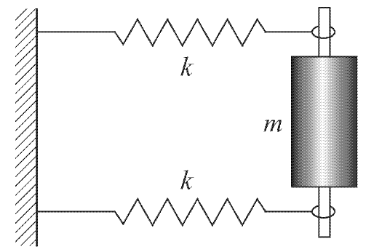
\includegraphics[width=0.3\textwidth]{rollOscil.png}
\caption{}
\label{rollOscil}
\vspace{0.2cm}
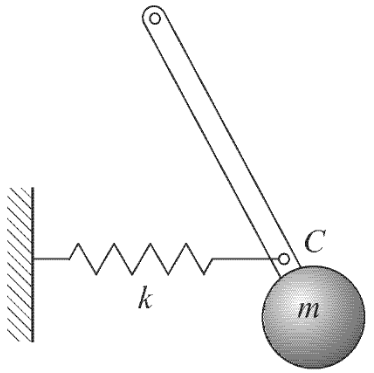
\includegraphics[width=0.3\textwidth]{physPend.png}
\caption{}
\label{physPend}
\vspace{0.2cm}
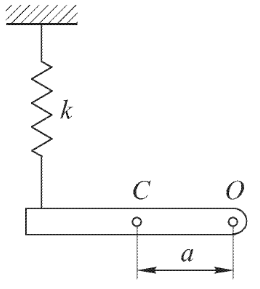
\includegraphics[width=0.3\textwidth]{springRodOsc.png}
\caption{}
\label{springRodOsc}
\end{wrapfigure}
%Сив602
\AddProb На горизонтальной плоскости находится цилиндр с моментом инерции $I$ (относительно продольной геометрической оси), массой $m$ и радиусом $r$. К оси цилиндра прикреплены две одинаковые горизонтально расположенные спиральные пружины, другие концы которых закреплены в стене (рис. \ref{rollOscil}, вид сверху). 
Коэффициент жесткости каждой пружины равен $k$; пружины могут работать как на растяжение, так и на сжатие. Найти период малых колебаний цилиндра, которые возникнут, если вывести его из положения равновесия и дать возможность кататься без скольжения по горизонтальной плоскости.
%Сив607
\AddProb Найти период малых колебаний физического маятника массы $m$, к центру масс $C$ которого прикреплена горизонтальная спиральная пружина с коэффициентом жесткости $k$. Другой конец пружины закреплен в неподвижной стенке (рис. \ref{physPend}). Момент инерции маятника относительно точки подвеса равен $I$, расстояние между точкой подвеса и центром масс маятника равно $a$. В положении равновесия пружина не деформирована.
%Сив607
\AddProb Колебательная система состоит из однородного стержня длины $l$ и массы $m$, который может вращаться вокруг горизонтальной оси $O$, проходящей через его конец и перпендикулярной к продольной оси стержня (рис. \ref{springRodOsc}). Другой конец стержня подвешен на пружине с коэффициентом жесткости $k$. Расстояние между серединой стержня и осью вращения $CO = a$. Момент инерции стержня относительно оси $O$ равен $I$. Найти удлинение пружины $x_0$ (по сравнению с ее длиной в недеформированном состоянии) в положении равновесия, если в этом $O$ положении стержень горизонтален. Определить также период малых колебаний стержня около положения равновесия.
%Сив587
\AddProb Однородная палочка подвешена за оба конца на двух одинаковых нитях длины $L$. В состоянии равновесия обе нити параллельны. Найти период $T$ малых колебаний, возникающих после некоторого поворота палочки вокруг вертикальной оси, проходящей через середину палочки.
%Сив592
\AddProb Сплошной однородный диск с радиусом $r = 10$ см колеблется около оси, перпендикулярной к плоскости диска и проходящей через край диска. Какой длины $l$ должен быть математический маятник, имеющий тот же период колебаний, что и диск?

\begin{wrapfigure}[10]{R}{2cm}
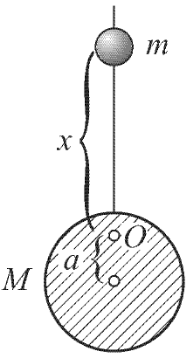
\includegraphics[width=0.15\textwidth]{metronom.png}
\caption{}
\label{metronom}
\end{wrapfigure}
%Сив598
\AddProb Маятник метронома представляет собой груз $M$, качающийся около оси $O$, с прикрепленной к нему спицей, по которой может перемещаться малый груз m (рис. \ref{metronom}). Как зависит период колебаний маятника от координаты $x$ грузика? Массу $m$ считать точечной. Момент инерции маятника метронома относительно оси $O$ равен $I$.
%Сив605
\AddProb Шарик массы $m$ подвешен на двух последовательно соединенных пружинках с коэффициентами жесткости $k_1$ и $k_2$. Определить период его вертикальных колебаний.
%Сив610
\AddProb Два незакрепленных шарика с массами $m_1$ и $m_2$ соединены друг с другом спиральной пружинкой с коэффициентом жесткости $k$. Определить период колебаний шариков относи-
относительно центра масс системы, которые возникнут при растяжении пружинки.

\begin{wrapfigure}[7]{R}{5cm}
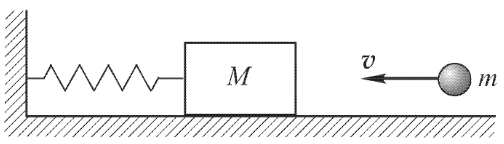
\includegraphics[width=0.4\textwidth]{shootOsc.png}
\caption{}
\label{shootOsc}
\end{wrapfigure}
%Сив619
\AddProb На горизонтальной пружине укреплено тело массы $M = 10$ кг, лежащее на гладком столе, по которому оно может скользить без 
трения (рис. \ref{shootOsc}). В это тело попадает и застревает в нем пуля массы $m = 10$ г, летящая с горизонтальной скоростью $v =
= 500$ м/с, направленной вдоль оси пружины. Тело вместе с застрявшей в нем пулей отклоняется от положения равновесия и начинает колебаться относительно него с амплитудой $A = 10$ см. Найти период колебаний тела.
\clearpage